\documentclass[11pt]{article}
\usepackage{homework}

\classname{364}
\homeworknum{5}


\DeclareMathAlphabet{\mathsfit}{T1}{\sfdefault}{\mddefault}{\sldefault}



\begin{document}

% Environments

\newcommand{\state}[2]{\begin{statement}{#1} #2 \end{statement}}
\newcommand{\prob}[2]{\begin{problem}{#1} #2 \end{problem}}
\newcommand{\subprob}[1]{\begin{subproblem} #1 \end{subproblem}}
\newcommand{\sol}[1]{\begin{solution} #1 \end{solution}}
\newcommand{\fig}[2]{\begin{figure} \centering #2  \label{#1} \end{figure}}

\newcommand{\makebib}{
	\vfill
	\color{black}
	\nocite{*}
	\bibliography{references}{}
	\bibliographystyle{lucas_unsrt}
}
	

% Implication

\newcommand{\qwhere}{\quad \text{where} \quad}
\newcommand{\qimplies}{\quad \implies \quad}
\newcommand{\impliesq}{\implies \quad}



% Brackets

\newcommand{\paren}[1]{\left( #1 \right)}
\newcommand{\brac}[1]{\left[ #1 \right]}
\newcommand{\curly}[1]{\left\{ #1 \right\}}


% Greek

\newcommand{\alp}{\alpha}
\newcommand{\bet}{\beta}
\newcommand{\gam}{\gamma}
\newcommand{\del}{\delta}
\newcommand{\eps}{\epsilon}
\newcommand{\zet}{\zeta}
\newcommand{\tht}{\theta}
\newcommand{\kap}{\kappa}
\newcommand{\lam}{\lambda}
\newcommand{\sig}{\sigma}
\newcommand{\ups}{\upsilon}
\newcommand{\omg}{\omega}

\newcommand{\Gam}{\Gamma}
\newcommand{\Del}{\Delta}
\newcommand{\Tht}{\Theta}
\newcommand{\Lam}{\Lambda}
\newcommand{\Sig}{\Sigma}
\newcommand{\Omg}{\Omega}


% Text

\newcommand{\where}{\text{where }}

% Problem 1

\newcommand{\Hint}{H_\text{int}}
\newcommand{\ddcx}{\dd[3]{x}}
\newcommand{\psib}{\bar{\psi}}

\newcommand{\mh}{m_h}
\newcommand{\mmu}{m_\mu}
\newcommand{\me}{m_e}
\newcommand{\ma}{m_a}

\newcommand{\aexpt}{a_\text{expt.}}
\newcommand{\aQED}{a_\text{QED}}
\renewcommand{\GeV}{\giga\electronvolt}

\newcommand{\gamt}{\gam^5}



\state{Ocean tides~(MCP 25.9)}{\hfix}

\prob{
	Place a local Lorentz frame at the center of Earth, and let $\cEsjk$ be the tidal field there, produced by the Newtonian gravitational fields of the Sun and the Moon.  For simplicity, treat Earth as precisely spherical.  Show that the gravitational acceleration (relative to Earth's center) at some location on or near Earth's surface (radius $r$) is
	\eq{
		\gsj = -\frac{G M}{r^2} \nj - \cEjsk r \nk,
	}
	where $M$ is Earth's mass, and $\nj$ is a unit vector pointing from Earth's center to the location at which $\gsj$ is evaluated.
}



\prob{
	Show that this gravitational acceleration is minus the gradient of the Newtonian potential
	\eq{
		\Phi = -\frac{G M}{r} + \frac{1}{2} \cEsjk r^2 \nj \nk.
	}
}



\prob{
	Consider regions of Earth's oceans that are far from any coast and have ocean depth large compared to the heights of ocean tides.  If Earth were nonrotating, then explain why the analysis of Sec~13.3 predicts that the ocean surface in these regions would be a surface of constant $\Phi$.  Explain why this remains true to good accuracy also for the rotating Earth.
}



\prob{
	Show that in these ocean regions, the Moon creates high tides pointing toward and away from itself and low tides in the transverse directions on Earth; and similarly for the Sun.  Compute the difference between high and low tides produced by the Moon and by the Sun, and the difference of the total tide when the Moon and the Sun are in approximately the same direction in the sky.  Your answers are reasonably accurate for deep-ocean regions far from any coast, but near a coast, the tides are typically larger and sometimes far larger, and they are shifted in phase relative to the positions of the moon and Sun.  Why?
}






\clearpage
\state{Components of the Riemann tensor in an arbitrary basis~(MCP 25.11)}{
	By evaluating expressions~(25.30) in an arbitrary basis (which might not even be a coordinate basis), derive Eq.~(25.50) for the components of the Riemann tensor.  In your derivation keep in mind that commas denote partial derivations \emph{only} in a coordinate basis; in an arbitrary basis they denote the result of letting a basis vector act as a differential operator.
}

\sol{
	MCP~(25.30) is
	\eqn{given2}{
		\fv{p}{\alp}{; \gam \del} - \fv{p}{\alp}{; \del \gam} = -\fv{R}{\alp}{\bet \gam \del} p^\bet,
	}
	where $\vp$ is any vector field.  MCP~(25.50) is
	\eqn{show2}{
		\fv{R}{\alp}{\bet \gam \del} = \fv{\Gam}{\alp}{\bet \del, \gam} - \fv{\Gam}{\alp}{\bet \gam, \del} + \fv{\Gam}{\alp}{\mu \gam} \fv{\Gam}{\mu}{\bet \del} - \fv{\Gam}{\alp}{\mu \del} \fv{\Gam}{\mu}{\bet \gam} - \fv{\Gam}{\alp}{\bet \mu} \sfv{c}{\gam \del}{\mu},
	}
	where $\Gasbg$ are the connection coefficients in the chosen basis, $\fv{\Gam}{\alp}{\bet \gam, \del}$ is the result of letting the basis vector $\ve_\del$ act as a differential operator on $\Gasbg$, and $\sfv{c}{\gam \del}{\mu}$ are the basis vectors' commutation coefficients.
	
	Beginning from Eq.~\refeq{given2},
	\al{
		\fv{R}{\alp}{\bet \gam \del} p^\bet &= \fv{p}{\alp}{; \del \gam} - \fv{p}{\alp}{; \gam \del} \\[1ex]
		&= \nabsg \fv{p}{\alp}{; \del} - \nabsd \fv{p}{\alp}{; \gam} \\[1ex]
		&= \fv{p}{\alp}{; \del , \gam} + \fv{p}{\nu}{; \del} \fv{\Gam}{\alp}{\nu \gam} - \fv{p}{\alp}{; \gam , \del} - \fv{p}{\mu}{; \gam} \fv{\Gam}{\alp}{\mu \del} \\[1ex]
		&= (\fv{p}{\alp}{, \del} + p^\sig \fv{\Gam}{\alp}{\sig \del})_{, \gam} + (\fv{p}{\nu}{, \del} + p^\tau \fv{\Gam}{\nu}{\tau \del}) \fv{\Gam}{\alp}{\nu \gam} - (\fv{p}{\alp}{, \gam} + p^\lam \fv{\Gam}{\alp}{\lam \gam})_{, \del} - (\fv{p}{\mu}{, \gam} + p^\rho \fv{\Gam}{\mu}{\rho \gam}) \fv{\Gam}{\alp}{\mu \del} \\[1ex]
		%
		&= \fv{p}{\alp}{, \del \gam} + \fv{p}{\sig}{, \gam} \fv{\Gam}{\alp}{\sig \del} + p^\sig \fv{\Gam}{\alp}{\sig \del, \gam} + \fv{p}{\nu}{, \del} \fv{\Gam}{\alp}{\nu \gam} + p^\tau \fv{\Gam}{\nu}{\tau \del} \fv{\Gam}{\alp}{\nu \gam} \\
		&\hspace{5em} \phantom{=\ } - \fv{p}{\alp}{, \gam \del} - \fv{p}{\lam}{, \del} \fv{\Gam}{\alp}{\lam \gam} - p^\lam \fv{\Gam}{\alp}{\lam \gam, \del} - \fv{p}{\mu}{, \gam} \fv{\Gam}{\alp}{\mu \del} - p^\rho \fv{\Gam}{\mu}{\rho \gam} \fv{\Gam}{\alp}{\mu \del} \\[1ex]
		%
		&= p^\sig \fv{\Gam}{\alp}{\sig \del, \gam} + p^\tau \fv{\Gam}{\nu}{\tau \del} \fv{\Gam}{\alp}{\nu \gam} - p^\lam \fv{\Gam}{\alp}{\lam \gam, \del} - p^\rho \fv{\Gam}{\mu}{\rho \gam} \fv{\Gam}{\alp}{\mu \del} \\
		&= (\fv{\Gam}{\alp}{\bet \del, \gam} - \fv{\Gam}{\alp}{\bet \gam, \del} + \fv{\Gam}{\alp}{\mu \gam} \fv{\Gam}{\mu}{\bet \del} - \fv{\Gam}{\alp}{\mu \del} \fv{\Gam}{\mu}{\bet \gam}) p^\bet
	}
	\hl{what happend to the connection coefficients???}
	
	where we have applied MCP~(24.35),
	\eqn{thing2}{
		\fv{A}{\mu}{; \bet} = \fv{A}{\mu}{, \bet} + A^\alp \fv{\Gam}{\mu}{\alp \bet}.
	}

%	Beginning from Eq.~\refeq{given2},
%	\eqn{thing2}{
%		\fv{R}{\alp}{\bet \gam \del} p^\bet = \fv{p}{\alp}{; \del \gam} - \fv{p}{\alp}{; \gam \del}
%		= \nabsg \fv{p}{\alp}{; \del} - \nabsd \fv{p}{\alp}{; \gam}
%		= \fv{p}{\alp}{; \del , \gam} + \fv{p}{\nu}{; \del} \fv{\Gam}{\alp}{\nu \gam} - \fv{p}{\alp}{; \gam , \del} - \fv{p}{\mu}{; \gam} \fv{\Gam}{\alp}{\mu \del},
%	}
%	where we have applied MCP~(24.35),
%	\eqn{thing2}{
%		\fv{A}{\mu}{; \bet} = \fv{A}{\mu}{, \bet} + A^\alp \fv{\Gam}{\mu}{\alp \bet}.
%	}
%	Now using MCP~(24.38c),
%	\eq{
%		\Gam_{\alp \bet \gam} = \frac{1}{2} (\sg_{\alp \bet, \gam} + \sg_{\alp \gam, \bet} - \sg_{\bet \gam, \alp} + c_{\alp \bet \gam} + c_{\alp \gam \bet} - c_{\bet \gam \alp})
%	}
%	and the fact that $\Gam_{\alp \bet \gam}$ is symmetric in its last two indices in a coordinate basis where the $c$ terms vanish~\cite[p.~1171]{MCP}, we can add to Eq.~\refeq{thing2}
%	\al{
%		0 &= \fv{p}{\alp}{; \zet} (\fv{\Gam}{\zet}{\gam \del} - \fv{c}{\zet}{\gam \del} - \fv{c}{\zet}{\del \gam} + c_\del{}^\zet{}_\gam) - \fv{p}{\alp}{; \eta} (\fv{\Gam}{\eta}{\del \gam} - \fv{c}{\eta}{\del \gam} - \fv{c}{\eta}{\gam \del} + c_\gam{}^\eta{}_\del) \\
%		&= \fv{p}{\alp}{; \zet} \fv{\Gam}{\zet}{\gam \del} - \fv{p}{\alp}{; \eta} \fv{\Gam}{\eta}{\del \gam} + \fv{p}{\alp}{; \xi} (-\fv{c}{\xi}{\gam \del} - \fv{c}{\xi}{\del \gam} + c_\del{}^\xi{}_\gam + \fv{c}{\xi}{\del \gam} + \fv{c}{\xi}{\gam \del} - c_\gam{}^\xi{}_\del) \\
%		&= \fv{p}{\alp}{; \zet} \fv{\Gam}{\zet}{\gam \del} - \fv{p}{\alp}{; \eta} \fv{\Gam}{\eta}{\del \gam} + \fv{p}{\alp}{; \xi} (c_\del{}^\xi{}_\gam - c_\gam{}^\xi{}_\del)
%	}

	\cite[p.~122]{Carroll}
}






\clearpage
\state{Weyl curvature tensor~(MCP 25.12)}{
	Show that the Weyl curvature tensor~(25.48) has vanishing contraction on all its slots and has the same symmetries as Riemann: Eqs.~(25.45).  From these properties, show that Weyl has just 10 independent components.  Write the Riemann tensor in terms of the Weyl tensor, the Ricci tensor, and the scalar curvature.
}

\sol{
	MCP~(24.28) is
	\eq{
		\fv{C}{\mu \nu}{\rho \sig} = \fv{R}{\mu \nu}{\rho \sig} - 2 \fv{\sg}{[ \mu}{[ \rho} \fv{R}{\nu ]}{\sig ]} + \frac{1}{3} \fv{\sg}{[ \mu}{[ \rho} \fv{\sg}{\nu ]}{\sig ]} R,
	}
	where the square brackets denote antisymmetrization, $A_{[ \alp \bet ]} = (A_{\alp \bet} - A_{\bet \alp}) / 2$, and $R = \fv{R}{\alp}{\alp}$.
}






\clearpage
\state{Curvature of the surface of a sphere~(MCP 25.13)}{
	On the surface of a sphere, such as Earth, introduce spherical polar coordinates in which the metric, written as a line element, takes the form
	\eqn{given4}{
		\dds^2 = a^2 (\ddtht^2 + \sin^2\tht \ddphi^2),
	}
	where $a$ is the sphere's radius.
}

\prob{ \label{4a}
	Show (first by hand and then by computer) that the connection coefficients for the coordinate basis $\{ \pdv*{\tht}, \pdv*{\phi} \}$ are
	\aln{ \label{show4a}
		\Gamtspp &= -\sin\tht \cos\tht, &
		\Gampstp &= \Gampspt = \cot\tht, &
		\text{all others vanish}.
	}
}

\sol{
	We follow the procedure on pp.~1171--1172 of MCP for computing the connection coefficients.  We use (24.38c) to compute
	\eqn{Gamthing}{
		\Gam_{\alp \bet \gam} = \frac{1}{2} (\sg_{\alp \bet, \gam} + \sg_{\alp \gam, \bet} - \sg_{\bet \gam, \alp} + c_{\alp \bet \gam} + c_{\alp \gam \bet} - c_{\bet \gam \alp}),
	}
	where we know the commutation coefficients $c_{\alp \bet \gam}$ vanish in a coordinate basis~\cite[p.~1171]{MCP}.  We raise the first index using (24.38d),
	\eqn{Gamraise}{
		\fv{\Gam}{\mu}{\bet \gam} = \sg^{\mu \alp} \Gam_{\alp \bet \gam}.
	}
	According to MCP~(24.7), the invariant interval is defined
	\eq{
		\dds^2 = \sg_{\alp \bet} \Del x^\alp \Del x^\bet.
	}
	This means the metric tensor components can be read off of Eq.~\refeq{given4} as
	\aln{ \label{met4}
		\sgstt &= a^2, &
		\sgspp &= a^2 \sin^2\tht.
	}
	The only nonzero derivative is
	\eq{
		\sg_{\phi \phi, \tht} = 2 a^2 \sin\tht \cos\tht.
	}
	so only connection coefficients with some combination of $\{ \phi, \phi, \tht \}$ can be nonzero.  Applying Eq.~\refeq{Gamthing} to the possible candidates, we find
	\al{
		\Gam_{\tht \phi \phi} &= \frac{1}{2} (\sg_{\tht \phi, \phi} + \sg_{\tht \phi, \phi} - \sg_{\phi \phi, \tht}) = -a^2 \sin\tht \cos\tht, \\
		\Gam_{\phi \tht \phi} &= \frac{1}{2} (\sg_{\phi \tht, \phi} + \sg_{\phi \phi, \tht} - \sg_{\tht \phi, \tht}) = a^2 \sin\tht \cos\tht, \\
		\Gam_{\phi \phi \tht} &= \frac{1}{2} (\sg_{\phi \phi, \tht} + \sg_{\phi \tht, \phi} - \sg_{\phi \tht, \phi}) = a^2 \sin\tht \cos\tht.
	}
	The components of the inverse metric tensor are
	\al{
		\sgtt &= \frac{1}{a^2}, &
		\sgpp &= \frac{1}{a^2 \sin^2\tht}.
	}
	Now applying Eq.~\refeq{Gamraise}, we have
	\ans{\al{
		\Gamtspp &= \sgtt \Gam_{\tht \phi \phi} = -\sin\tht \cos\tht, &
		\Gampstp &= \sgpp \Gam_{\phi \tht \phi} = \cot\tht, &
		\Gampspt &= \sgpp \Gam_{\phi \phi \tht} = \cot\tht.
	}}%
	as we wanted to show. \qed
	
	By computer, we use a Mathematica notebook adapted from Ref.~\cite{Hartle}:
	
	\scalebox{0.625}{
		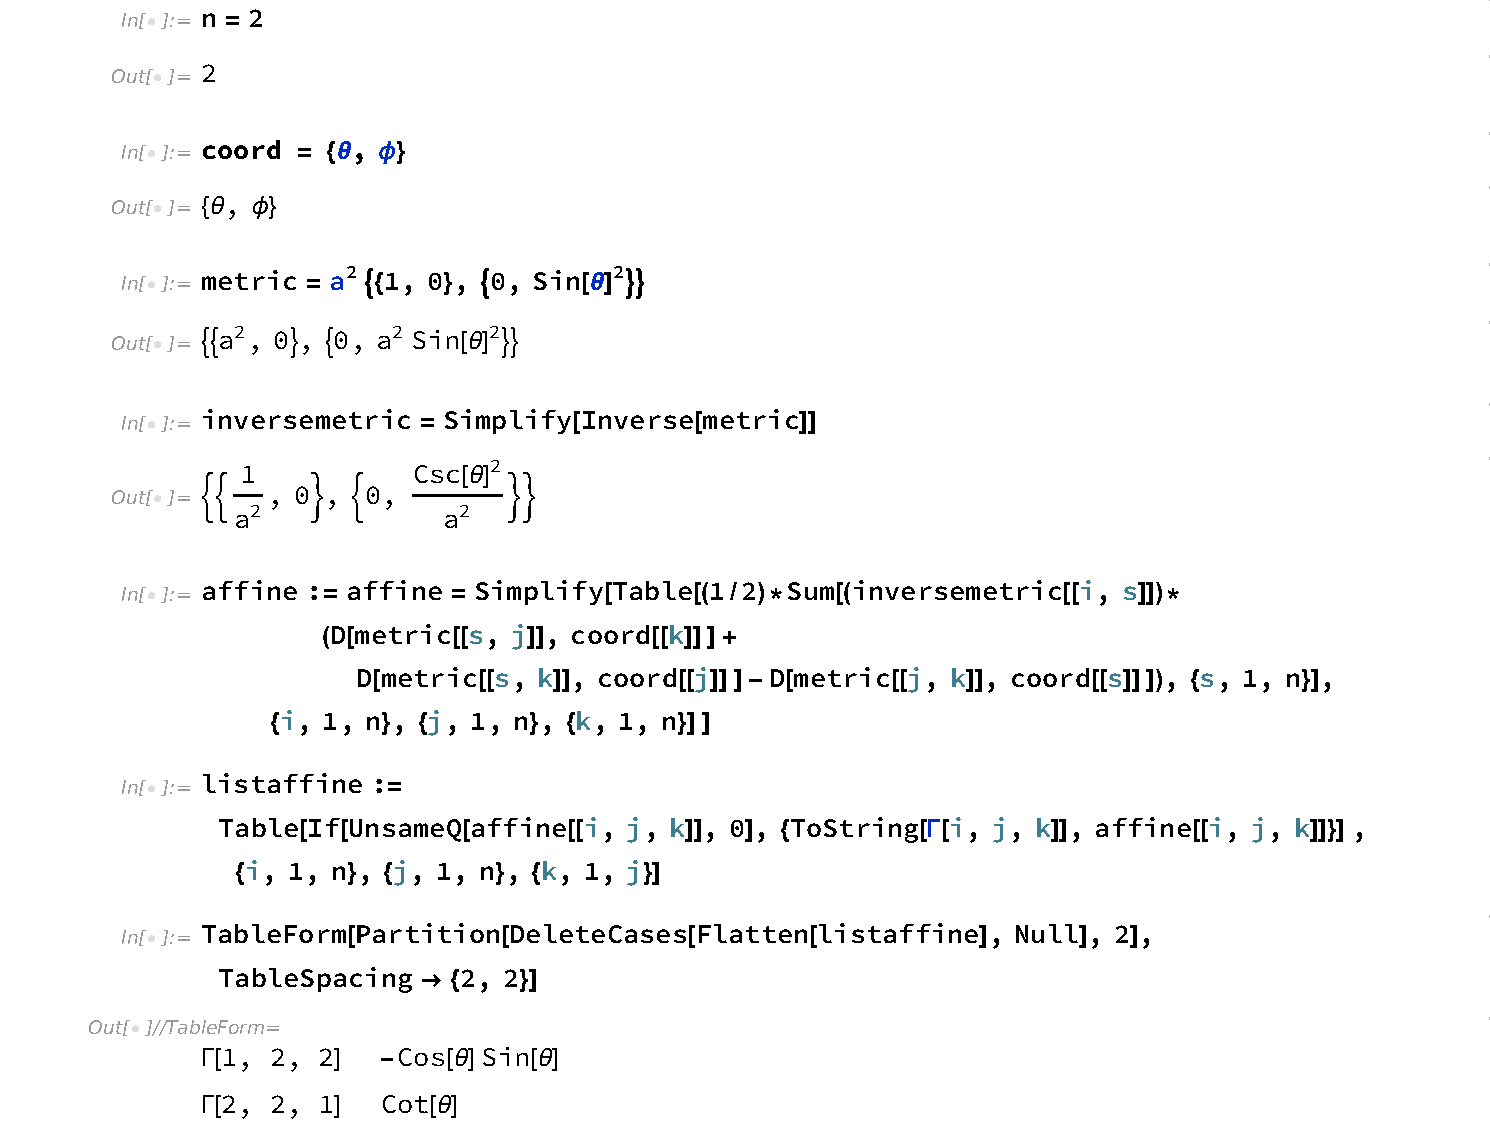
\includegraphics{4a}
	}
	
	Here $\tht \to 1$ and $\phi \to 2$.  Taking into account that in a coordinate basis $\Gam_{\alp \bet \gam}$ is symmetric in its last two indices~\cite[p.~1172]{MCP}, these match our result.
}



\prob{
	Show that the symmetries (25.45) of the Riemann tensor guarantee that its only nonzero components in the above coordinate basis are
	\eq{
		\Rstptp = \Rsptpt = -\Rstppt = -\Rspttp.
	}
}

\sol{
	According to MCP~(25.45a),
	\aln{ \label{symm}
		R_{\alp \bet \gam \del} &= -R_{\bet \alp \gam \del}, &
		R_{\alp \bet \gam \del} &= -R_{\alp \bet \del \gam}, &
		R_{\alp \bet \gam \del} &= +R_{\gam \del \alp \bet}.
	}
	Applying these to the six possible permutations of $\{ \tht, \tht, \phi, \phi \}$, we have
	\ans{\al{
		R_{\tht \tht \phi \phi} &= -R_{\tht \tht \phi \phi} = 0, &
		R_{\phi \phi \tht \tht} &= -R_{\phi \phi \tht \tht} = 0, &
		R_{\tht \phi \phi \tht} &= -R_{\phi \tht \phi \tht} = -R_{\tht \phi \tht \phi} = R_{\phi \tht \tht \phi},
	}}%
	as we wanted to show. \qed
}



\prob{
	Show, first by hand and then by computer, that
	\eq{
		\Rstptp = a^2 \sin^2\tht.
	}
}

\sol{
	From Eq.~\refeq{show2},
	\eq{
		\fv{R}{\tht}{\phi \tht \phi} = \fv{\Gam}{\tht}{\phi \phi, \tht} - \fv{\Gam}{\tht}{\phi \tht, \phi} + \fv{\Gam}{\tht}{\mu \tht} \fv{\Gam}{\mu}{\phi \phi} - \fv{\Gam}{\tht}{\mu \phi} \fv{\Gam}{\mu}{\phi \tht} - \fv{\Gam}{\tht}{\phi \mu} \sfv{c}{\tht \phi}{\mu}.
	}
	From Eq.~\refeq{show4a},
	\al{
		\fv{\Gam}{\tht}{\phi \phi, \tht} &= \sin^2\tht - \cos^2\tht, &
		\fv{\Gam}{\phi}{\tht \phi, \tht} &= \fv{\Gam}{\phi}{\phi \tht, \tht} = -\csc^2\tht, &
		\fv{\Gam}{\tht}{\phi \phi, \phi} &= \fv{\Gam}{\phi}{\tht \phi, \phi} = \fv{\Gam}{\phi}{\phi \tht, \phi} = 0.
	}
	We also know that all $c_{\alp \bet \gam} = 0$.  Equation~\refeq{thing4c} is then
	\eq{
		\fv{R}{\tht}{\phi \tht \phi} = \fv{\Gam}{\tht}{\phi \phi, \tht} - \fv{\Gam}{\tht}{\phi \phi} \fv{\Gam}{\phi}{\phi \tht}
		= \sin^2\tht - \cos^2\tht - (-\sin\tht \cos\tht) (\cot\tht)
		= \sin^2\tht.
	}
	Lowering the first index using Eq.~\refeq{met4}, we find
	\eq{
		\ans{ \Rstptp = \sgstt \fv{R}{\tht}{\phi \tht \phi}
		= a^2 \sin^2\tht }
	}
	as we wanted to show. \qed
	
	Continuing the notebook from \ref{4a},
	
	\scalebox{0.625}{
		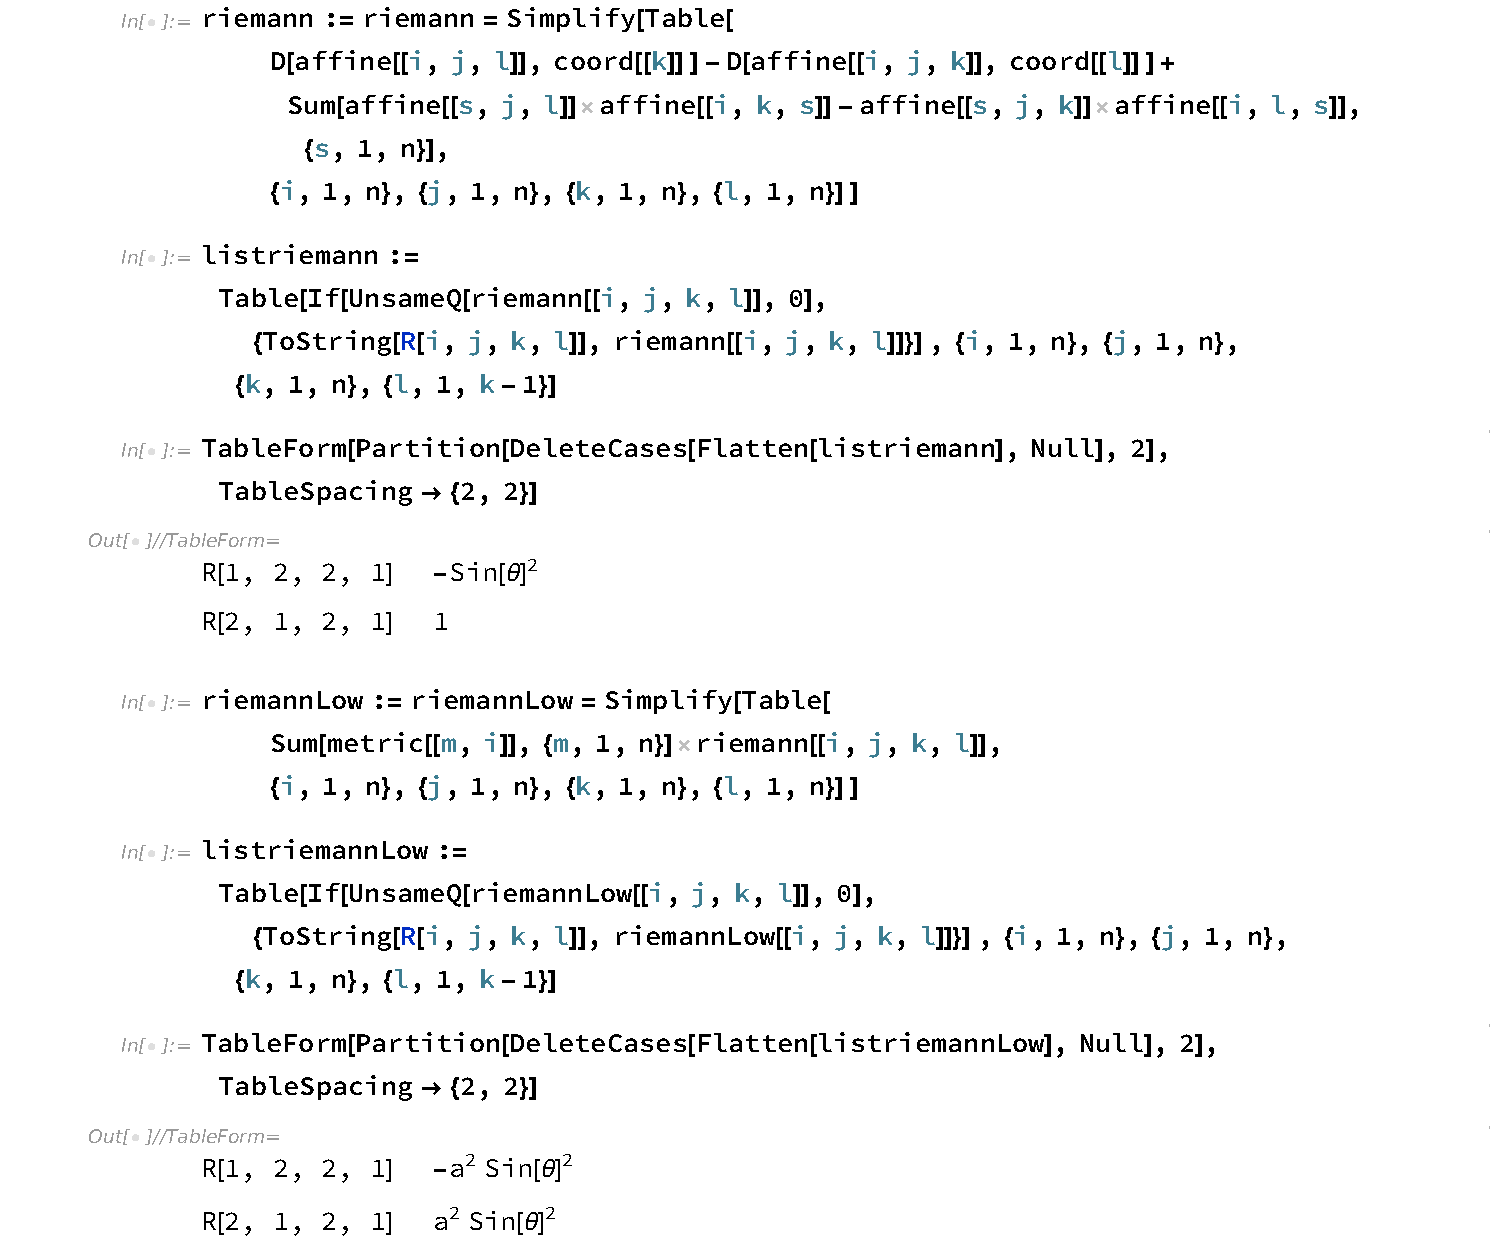
\includegraphics{4c}
	}
	
	Here the second list of \nolinkurl{R[_, _, _, _]} has the first index lowered.  By Eq.~\refeq{symm}, \nolinkurl{R[1, 2, 2, 1]} is equivalent to $\text{\nolinkurl{R[1, 2, 1, 2]}} \to \Rstptp$, which agrees with our calculation.
}



\prob{
	Show that in the basis
	\eq{
		\{ \vesthh, \vesphh \} = \curly{ \frac{1}{a} \pdv{\tht}, \frac{1}{a \sin\tht} \pdv{\phi} },
	}
	the components of the metric, the Riemann tensor, the Ricci tensor, the curvature scalar, and the Weyl tensor are
	\al{
		\sgsjhkh &= \delsjk, &
		\Rsthphthph &= \frac{1}{a^2}, &
		\Rsjhkh &= \frac{1}{a^2} \sgsjhkh, &
		R &= \frac{2}{a^2}, &
		\Csthphthph &= 0,
	}
	respectively.  The first of these implies that the basis is orthonormal; the rest imply that the curvature is independent of location on the sphere, as it should be by spherical symmetry.
}





\clearpage
\state{Geodesic deviation on a sphere~(MCP 25.14)}{
	Consider two neighboring geodesics (great circles) on a sphere of radius $a$, one the equator and the other a geodesic slightly displaced from the equator (by $\Del\tht = b$) and parallel to it at $\phi = 0$.  Let $\vxi$ be the separation vector betwen the two geodesics, and note that at $\phi = 0$, $\vxi = b \pdv*{\tht}$.  Let $l$ be proper distance along the equatorial geodesic, so $\dv*{l} = \vuu$ is its tangent vector.
}

\prob{
	Show that $l = a \phi$ along the equatorial geodesic.
}



\prob{
	Show that the equation of geodesic deviation (25.31) reduces to
	\aln{ \label{show5b}
		\dv[2]{\xit}{\phi} &= - \xit, &
		\dv[2]{\xip}{\phi} &= 0.
	}
	\vfix
}



\prob{
	Solve Eq.~\refeq{show5b}, subject to the above initial conditions, to obtain
	\al{
		\xit &= b \cos\phi, &
		\xip &= 0.
	}
	Verify, by drawing a picture, that this is precisely what one would expect for the separation vector between two great circles.
}





\clearpage
\state{Curvature-coupling torque~(MCP 25.16)}{\hfix}

\prob{
	In the Newtonian theory of gravity, consider an axisymmetric, spinning body (e.g., Earth) with spin angular momentum $\Sj$ an dtimei-independent mass distribution $\rho(\bx)$, interacting with an externally produced tidal gravitational field $\cEsjk$ (e.g., that of the Sun and the Moon).  Show that the torque around the body's center of mass, exerted by the tidal field, and the resulting evolution of the body's spin are
	\eqn{show6a}{
		\dv{\Ssi}{t} = -\epssijk \cIsjl \cEskl.
	}
	Here
	\eq{
		\cIskl = \int \rho \paren{ \xsk \xsl - \frac{1}{3} r^2 \delskl } \ddV
	}
	is the body's mass quadrupole moment, with $r = \sqrt{\delsij \xsi \xsj}$ the distance from the center of mass.
}



\prob{
	For the centrifugally flattened Earth interacting with the tidal fields of the Moon and the Sun, estimate in order of magnitude the spin-precession period produced by this torque.  [The observed precession period is 26,000 years.]
}



\prob{
	Show that when rewritten in the language of general relativity, and in frame-independent, geometric language, Eq.~\refeq{show6a} takes the form (25.59) discussed in the text.  As part of showing this, explain the meaning of $\cIsbm$ in that equation.
}

\makebib

\end{document}
